\documentclass{article}
\usepackage{xspace}
\usepackage{fancyhdr}
\usepackage{graphicx}
\usepackage{amsmath,amssymb,amsthm}
\usepackage{microtype}
\usepackage{enumitem}
\usepackage{ifthen}
\usepackage{totcount}
\usepackage{algpseudocode}
\usepackage[usenames,usedvpinames]{xcolor}
\usepackage[most]{tcolorbox}
\usepackage[a4paper, margin=1in]{geometry}
\usepackage{parskip}
\usepackage{float}
% \usepackage{subcaption}
\usepackage{caption}
\usepackage{subfloat}
\usepackage{subfig}

\graphicspath{ {./figures/} }

%--------------------------------------------------------------------------------

\newcommand{\edition}{2022-2023}
\newcommand{\deadline}{14 December 2022, 11:00}
\newcommand{\hwNum}{2}

\newcommand{\student}{Alexander Apers \\ 6272932}

%--------------------------------------------------------------------------------
% Style stuff
\pagestyle{fancy}
\lhead{Geometric Algorithms (INFOGA \edition)}
\chead{}
\rhead{\mytitle}
\lfoot{INFOGA \edition}
\cfoot{\student}
\rfoot{\thepage}
\renewcommand{\headrulewidth}{0.4pt}
\renewcommand{\footrulewidth}{0.4pt}
\renewcommand{\familydefault}{\sfdefault}

%--------------------------------------------------------------------------------
% Question macro's

\newcommand{\withpoints}[1]{%
  \addtocounter{pointscounter}{#1} \printpoints{#1}
}
\newcommand{\printpoints}[1]{%
   \ifthenelse{#1 = 0}
              {}
              {\textit{(#1 points)}}\mbox{}
}



\newenvironment{question}[1][0]{\begin{tcolorbox}[parbox=false
                                      ,breakable=true
                                      ,enhanced jigsaw
                                      ,title=\bfseries Question
                                      \stepcounter{questionscounter}\arabic{questionscounter}
                                      \withpoints{#1}]
                         }
                         {\end{tcolorbox}}
\newenvironment{subquestions}{\begin{enumerate}[leftmargin=*
                                        ]}
                             {\end{enumerate}}
\newcommand{\subquestion}[1][0]{\item \withpoints{#1}}

\newtotcounter{questionscounter}
\newtotcounter{pointscounter}

\newcommand{\numquestions}{\total{questionscounter}}
\newcommand{\numpoints}{\total{pointscounter}}

%--------------------------------------------------------------------------------
\newcommand{\myremark}[3]{\textcolor{blue}{\textsc{#1 #2:}} \textcolor{red}{\textsf{#3}}}
% \renewcommand{\myremark}[3]{}
\newcommand{\frank}[2][says]{\myremark{Frank}{#1}{#2}}

%--------------------------------------------------------------------------------
% Theorem Environments
\newtheorem{theorem} {Theorem}
\newtheorem{lemma}[theorem] {Lemma}
\newtheorem{corollary}[theorem] {Corollary}
\newtheorem{problem}[theorem] {Problem}
\newtheorem{observation}[theorem] {Observation}
\newtheorem{claim}[theorem] {Claim}
\newtheorem{invariant}[theorem] {Invariant}

%--------------------------------------------------------------------------------
% Otherwise useful Macro's
\newcommand{\eps}{\ensuremath{\varepsilon}\xspace}
\DeclareMathOperator{\argmin}{argmin}
\DeclareMathOperator{\argmax}{argmax}

\newcommand{\mkmbb}[1]{\ensuremath{\mathbb{#1}}\xspace}
\newcommand{\R}{\mkmbb{R}}

\newcommand{\mathfunc}[1]{\ensuremath{\mathit{#1}}\xspace}

%--------------------------------------------------------------------------------
% The Actual document

\newcommand{\mytitle}{Homework Exam \hwNum\xspace\edition}
\title{\mytitle}
\date{\textbf{Deadline: } \deadline}
\author{\student}


\begin{document}
\maketitle
\thispagestyle{fancy}
  \noindent
  This homework exam has \numquestions\xspace questions for a total of
  \numpoints\xspace points. You can earn 10 additional points by a
  careful preparation of your hand-in: using a good layout, good
  spelling, good figures, no sloppy notation, no statements like ``The
  algorithm runs in $n\log n$.''  (forgetting the $O(..)$ and
  forgetting to say that it concerns time), etc. Use lemmas, theorems,
  and figures where appropriate. Your final grade will be the number
  of points divided by 10. Unless stated otherwise, both randomized
  and deterministic solutions are allowed. In case you are asked to
  analyze the running time and your algorithm is randomized, analyze
  its expected running time.

  \begin{question}[20] Let $\mathcal{S}$ be a planar subdivision with
    $n$ vertices, represented as a DCEL. Give \emph{pseudo-code} for
    an output sensitive algorithm that, given a pointer to a face $F$,
    reports all $k$ half-edges that have a vertex in common with $F$.

    Your algorithm should use the 'Twin', 'NextEdge', 'PrevEdge',
    etc. fields to navigate (i.e. you cannot assume you can directly
    access a list of vertices). Describe in a few sentences the main
    idea of your algorithm and analyze its running time.
  \end{question}

  %  My answers for Q1 here...
  In my answers I used the interpretation that both a half-edge and its twin are incident to both vertices that the edge is between.
  Therefore, for every half-edge that will be added, its twin will be added as well. 

  The idea is to traverse every vertex that is in common with $F$. These vertices and the edges between the make up the OuterComponent and the InnerComponents. 
  Given a vertex $v$ that is in common with $F$, we want to report all of the half-edges that have $v$ as origin as well as their twins by the reasoning above.
  This is done in the \textproc{ReportHalfEdgesOfVertex} function. 
  Traversing the OuterComponent and InnerComponents is done in the \textproc{ReportHalfEdges} function. 
  This is done by starting at the given edge and using the Next and Origin fields consecutively to find the vertices that are in common with $F$. 

  The running time of this algorithm is $O(k)$. 
  Even though the algorithm does have nested loops, we know that the number of half-edges to report will be $O(k)$.
  Reporting a single half-edge can be done in $O(1)$ time.
  Since the algorithm doesn't do any additional work except for traversing the vertices to report the required half-edges, 
  we know the time complexity of the nested loops must be bounded by $O(k)$. \\

  \begin{algorithmic}
    \Function{ReportHalfEdges}{$F$} 
      \State $e_0 \gets F$.OuterComponent
      \State $e \gets e_0$
      \While{$e \neq e_0$.Prev}
        \State $v \gets e$.Origin
        \State \textproc{ReportHalfEdgesOfVertex}($v$)
        \State $e \gets e$.Next
      \EndWhile
      \State
      \For{InnerComponent $e_0$ in $F$.InnerComponents}
        \State $e \gets e_0$
        \While{$e \neq e_0$.Prev}
          \State $v \gets e$.Origin
          \State \textproc{ReportHalfEdgesOfVertex}($v$)
          \State $e \gets e$.Next
        \EndWhile
      \EndFor
    \EndFunction
  \end{algorithmic} 

  \vspace{.2cm}

  \begin{algorithmic}
    \Function{ReportHalfEdgesOfVertex}{$v$} 
      \State $e_0 \gets v$.IncidentEdge 
      \State $e \gets e_0$
      \While{$t \neq e_0$.Prev}
        \State \textproc{Report}(e)
        \State $t \gets e$.Twin
        \State \textproc{Report}(t)
        \State $e \gets t$.Next
      \EndWhile
    \EndFunction
  \end{algorithmic}
  

  \begin{question}
    \begin{subquestions}
      \subquestion[10] Show that a triangulation of a polygon with
      $n \geq 9$ vertices with $h {\color{red}{>}} 1$ holes may consist of more than $n$
      triangles. That is, describe a construction that, given a number
      $n \geq 9$, constructs a polygon $P_n$ with $n$ vertices that
      has a triangulation with more than $n$ triangles.

      \subquestion[15] Prove that any triangulation of a polygon $P$
      with $n$ vertices and $h$ holes actually has the same number of
      triangles.
    \end{subquestions}
  \end{question}

  %  My answers for Q2 here...
  \begin{enumerate}
    \item  We start by presenting a base case construction for $P_n$ with $n = 9$ and $h = 2$ that has a triangulation which consists of strictly more than $n$ triangles.
    Then we will show that $P_{n+1}$ can be constructed from $P_n$ using a simple procedure. $P_{n+1}$ will have a triangulation that has strictly more than $n+1$ triangles.
    Then by the principle of induction, given any $n \geq 9, n\in\mathbb{N}$ there exists a polygon $P_n$ with $n$ vertices and a triangulation with strictly more than $n$ triangles.

    \textbf{Base case construction} \\
    The construction for $P_9$ with $n=9$ vertices and $h=2$ holes is shown in Figure \ref{fig:original} along with a triangulation in Figure \ref{fig:triangulation}. 
    This triangulation consists of 11 triangles which is strictly more than 9.
    The outer boundary of the polygon and the holes are all triangles.
    
    \begin{figure}[H]
      \centering
        \subfloat[original $P_9$ \label{fig:original} ]{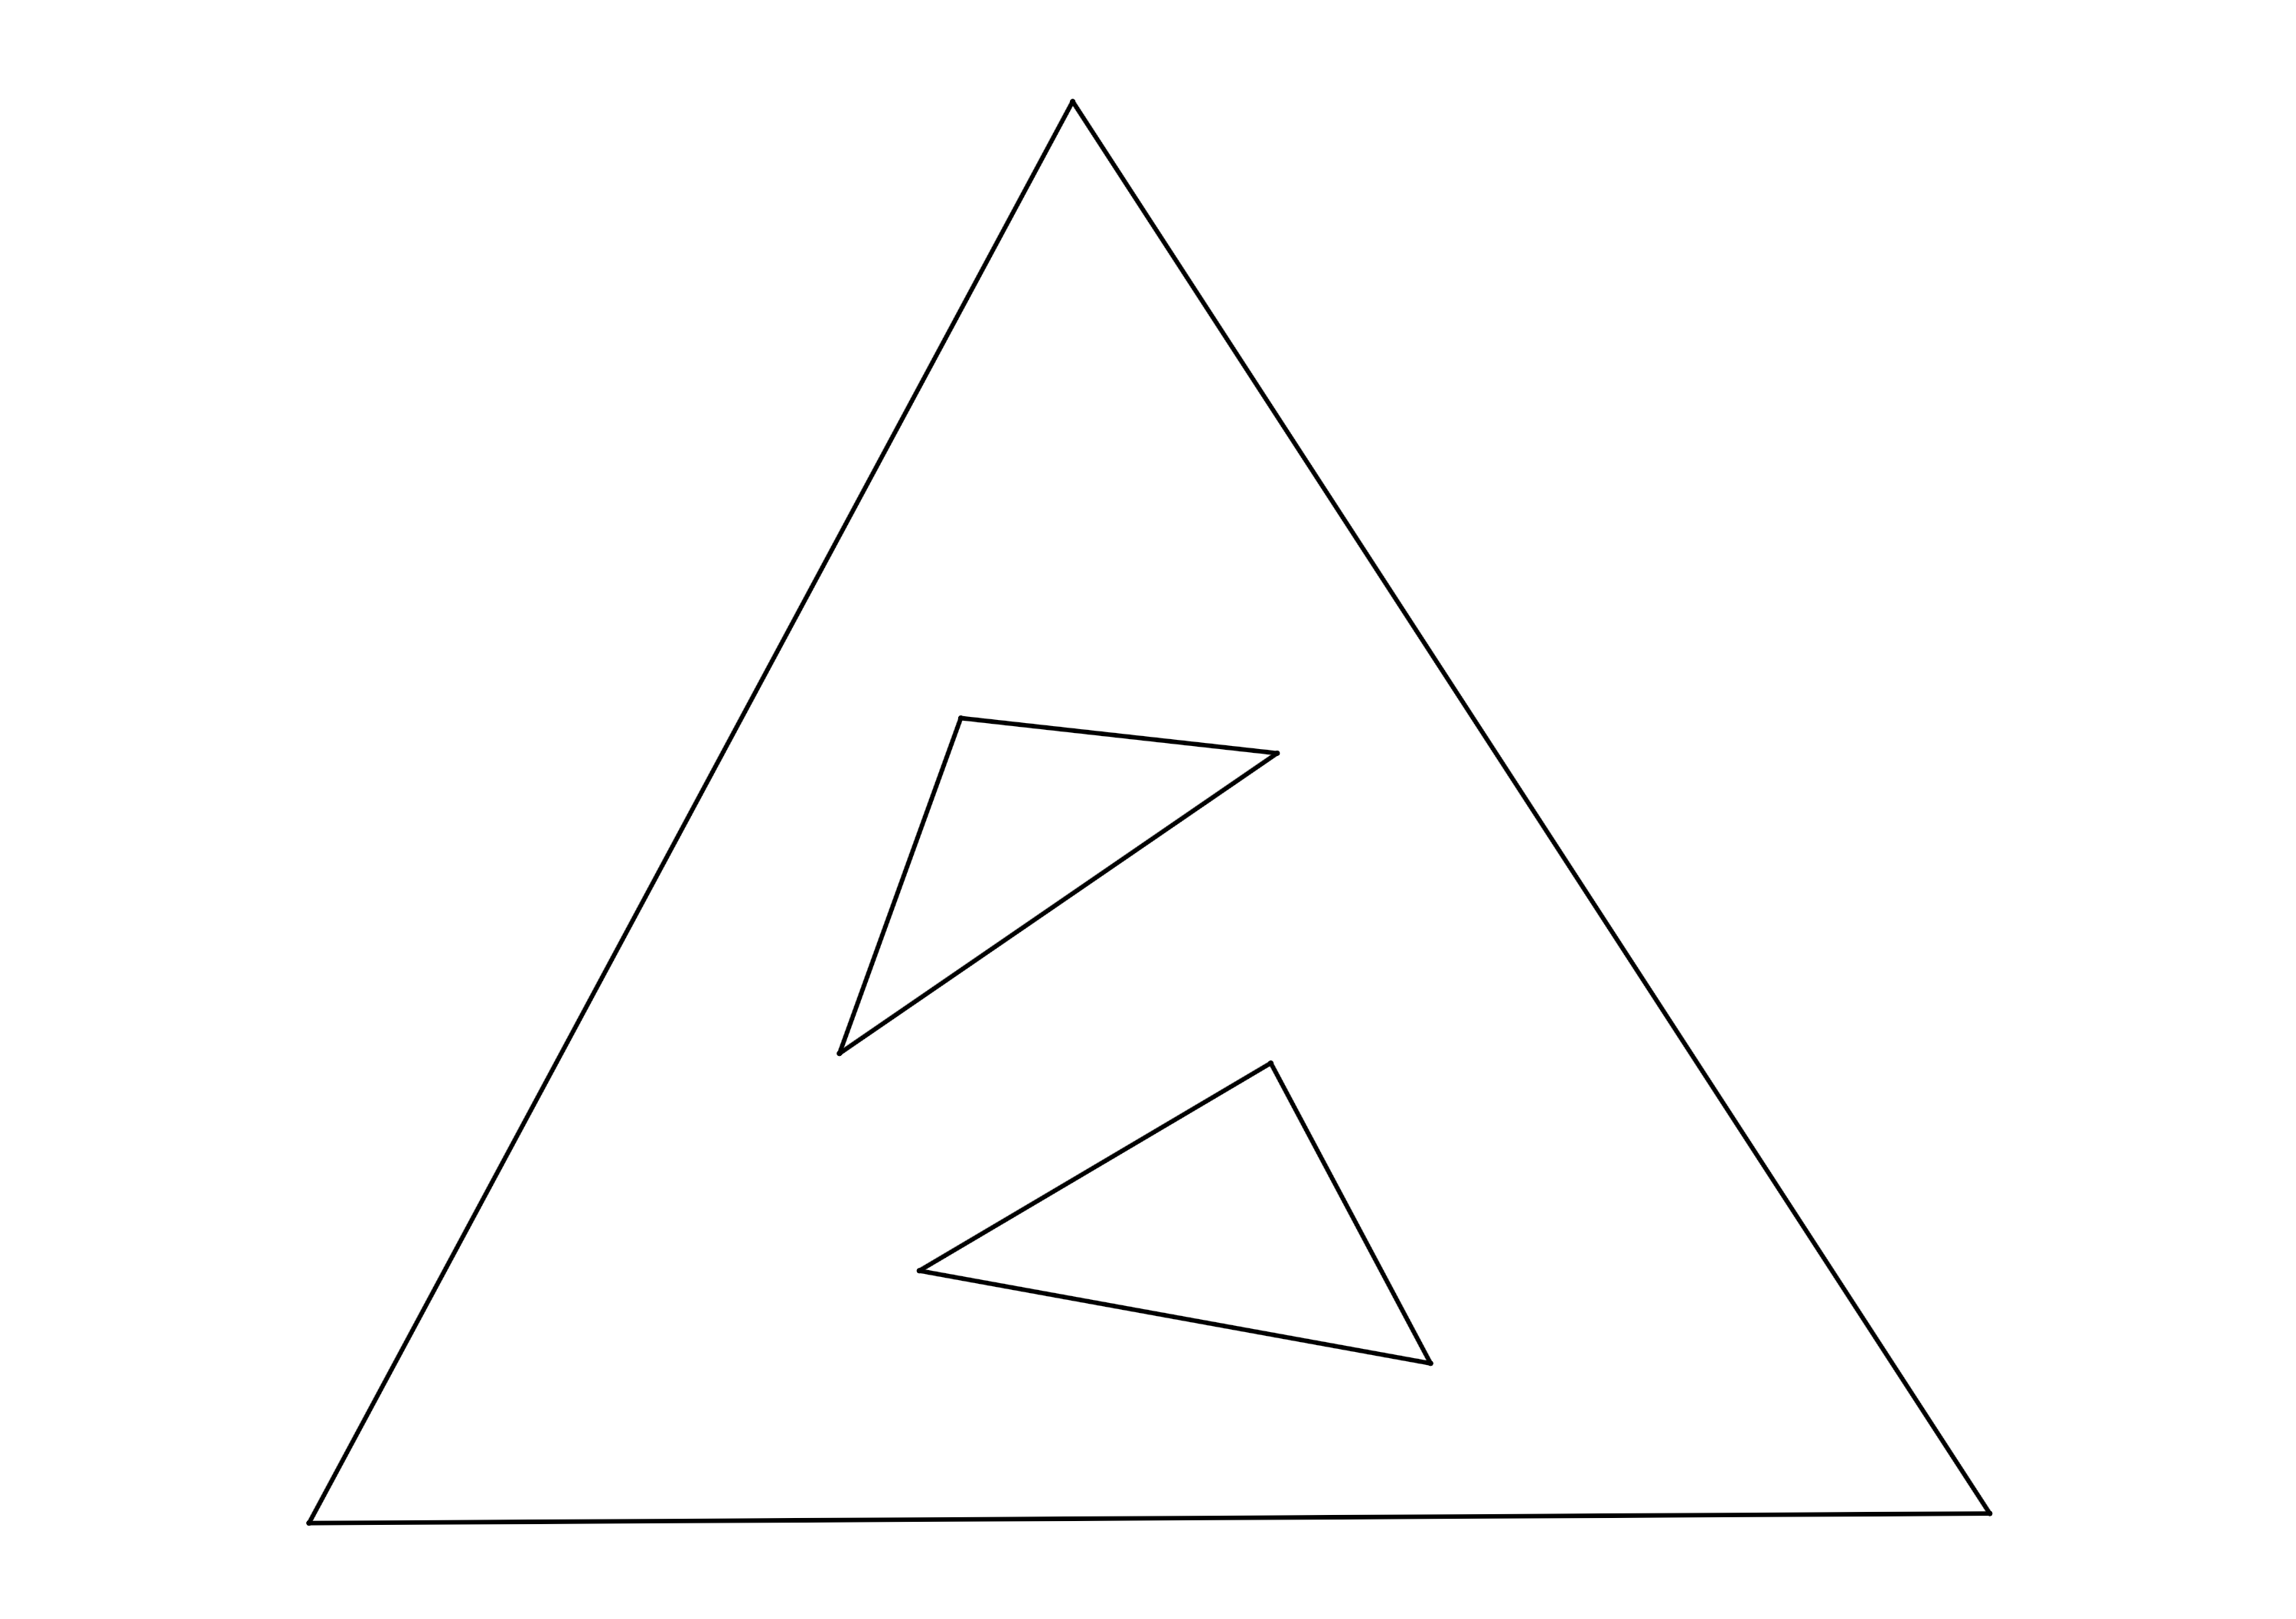
\includegraphics[width=.4\textwidth]{geogebra-export-7.png}\hspace{-.2cm}}
        \subfloat[triangulation of $P_9$ \label{fig:triangulation}]{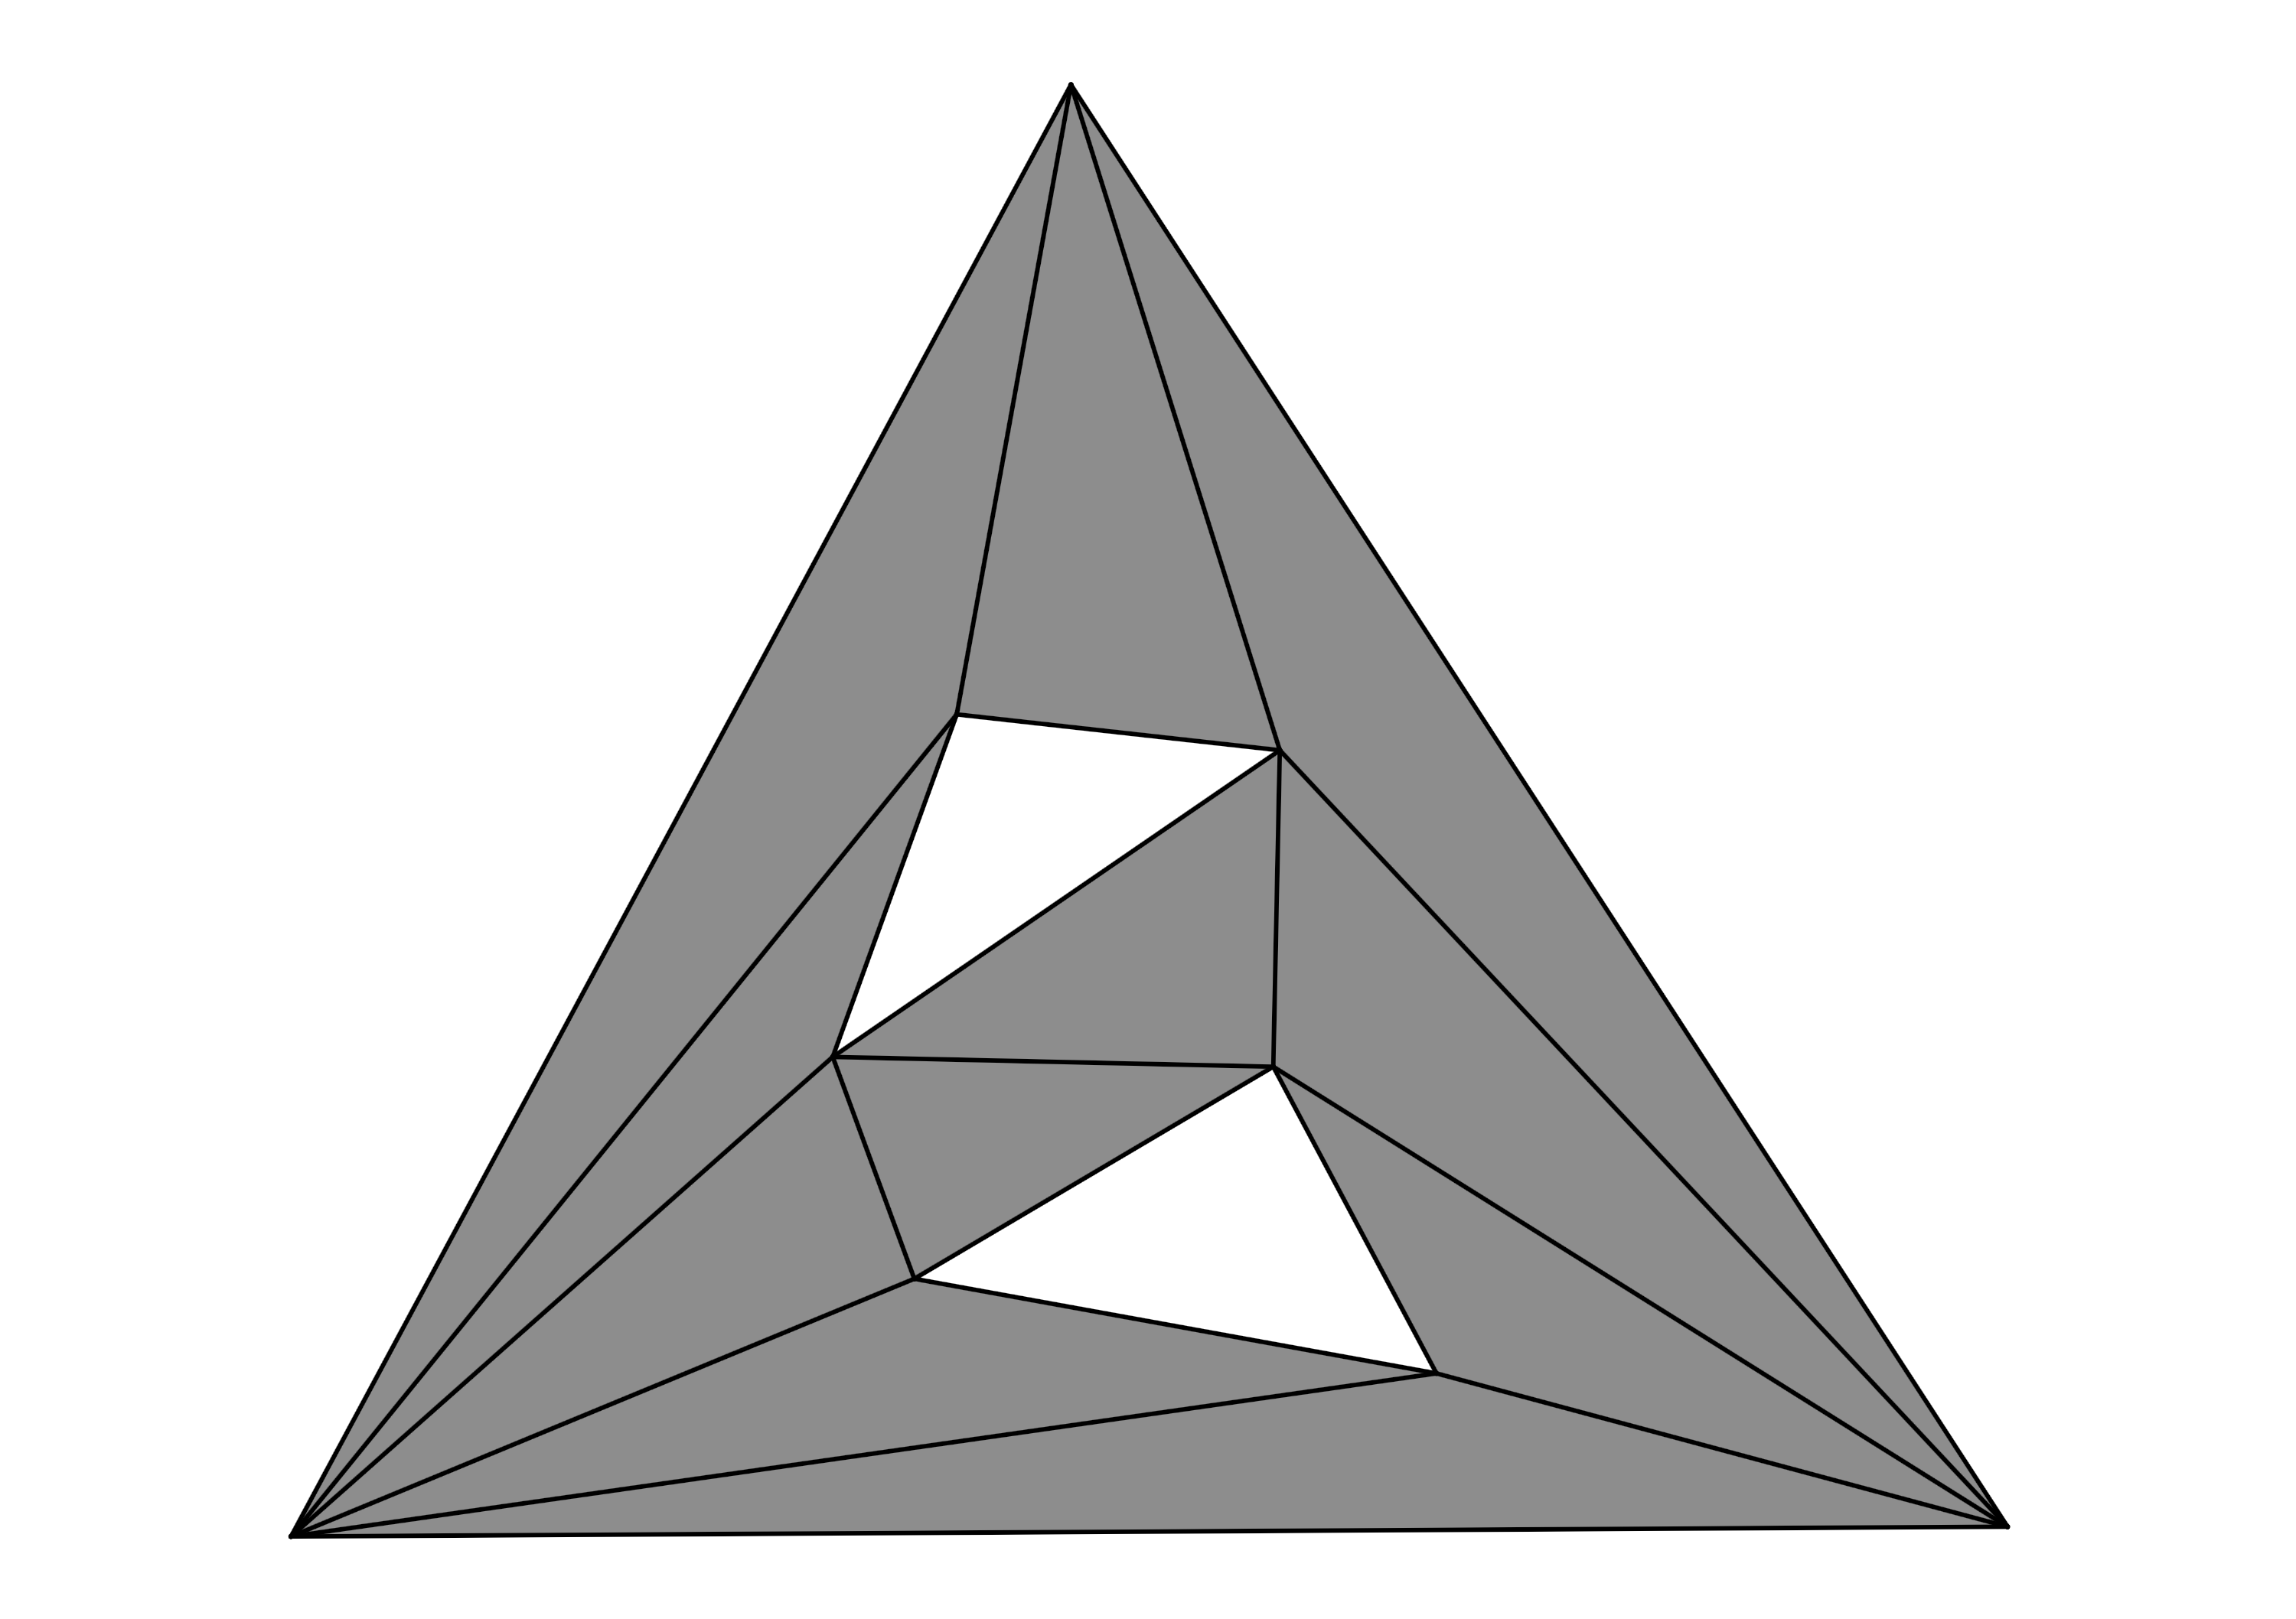
\includegraphics[width=.4\textwidth]{geogebra-export-8.png}}
        \caption{Polygon $P_9$ with $n=9$ vertices and $h=2$ holes} 
        \label{fig:p9}
      \end{figure}
  

    \textbf{Induction step} \\
    Assume we have a construction of $P_n$ with $n \geq 9$ with $n\in\mathbb{N}$ that has a triangulation with $x$ triangles with $x > n$.
    We construct $P_{n+1}$ by adding an additional vertex outisde of the outer boundary of $P_n$. 
    This will always add 1 or 2 triangles depending on the exact location of the new vertex. 
    This triangle or these triangles will consist of the new vertex that is added and two vertices that are connected by an edge in $P_n$. 
    These vertices are chosen so that the outer boundary of $P_n$ is not intersected. 

    $P_{n+1}$ will then have a triangulation with $x + 1$ or $x + 2$ triangles.
    Since by induction hypothesis $x > n$, it follows that both $x+1 > n+1$ and $x+2 > n+1$.

    To illustrate this we show an example. Figure \ref{fig:p10}a and b show two different constructions of $P_{10}$. In Figure \ref{fig:left} the new vertex is added to the left of $P_9$ which adds a single extra triangle.
    In Figure \ref{fig:top} the new vertex is added towards the top of $P_9$ which adds two extra triangles.

    \begin{figure}[H]
      \centering
        \subfloat[$P_{10}$ constructed from $P_9$ \label{fig:left}]{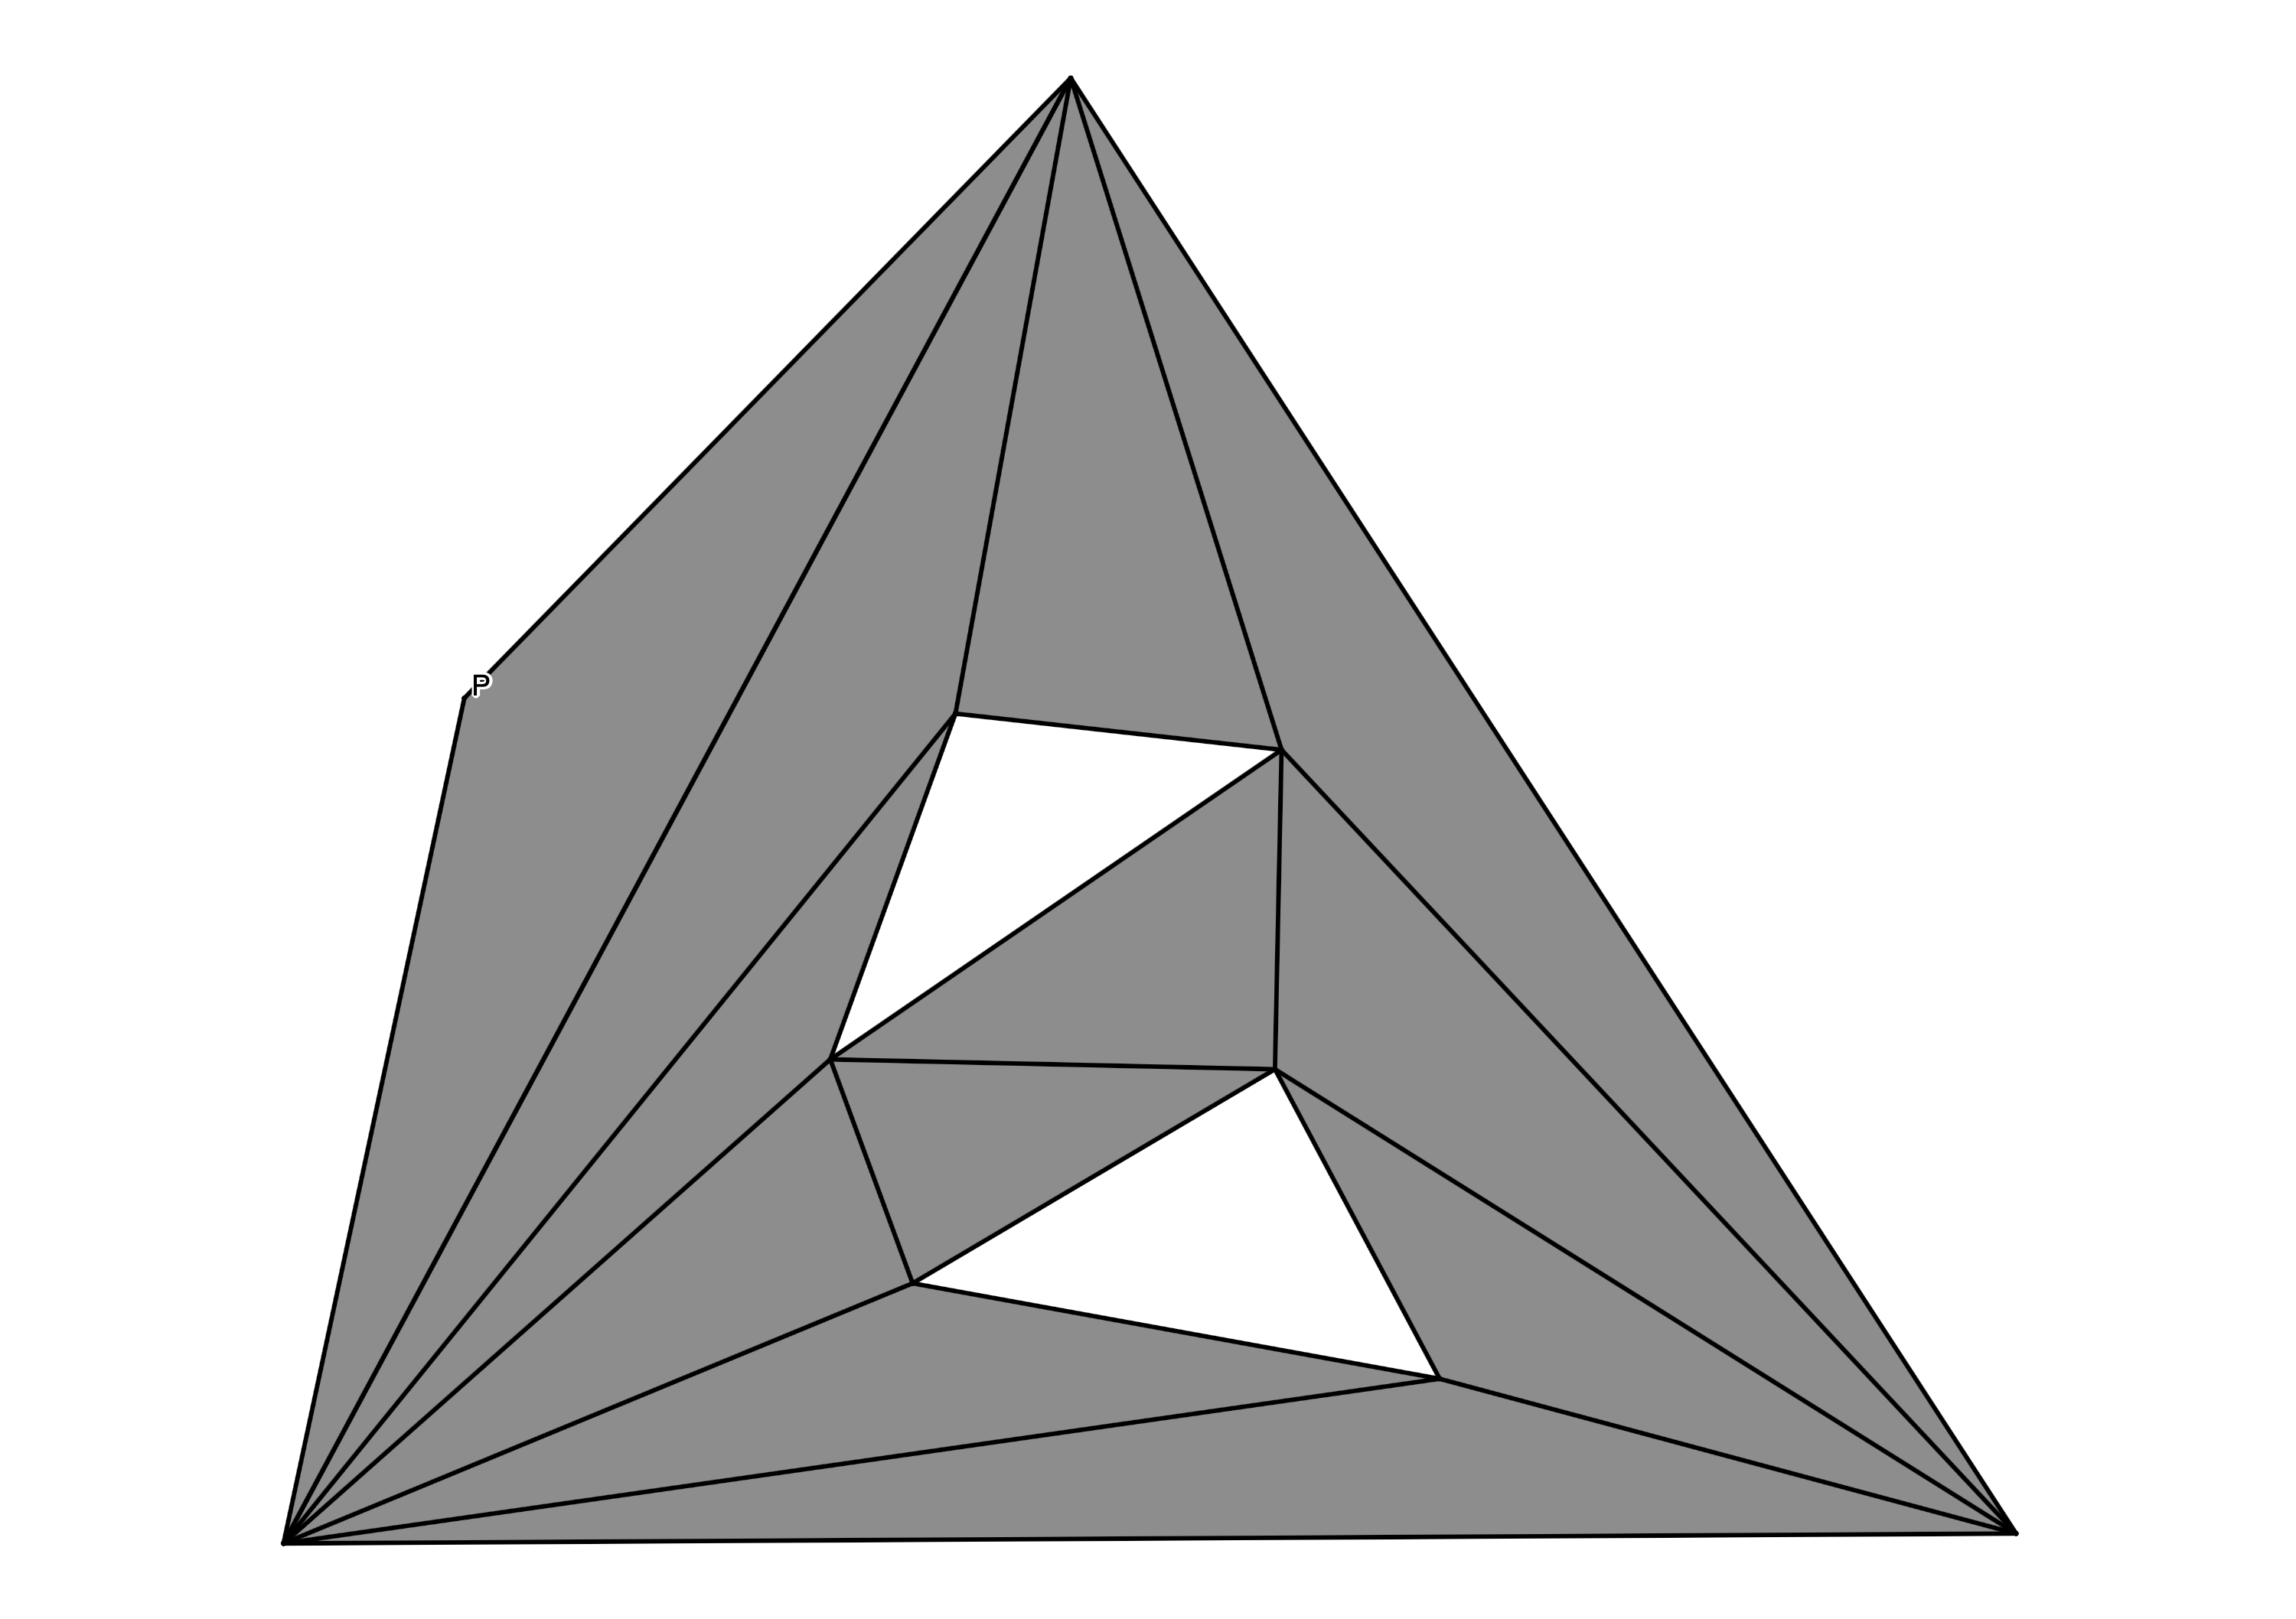
\includegraphics[width=.4\textwidth]{geogebra-export-10.png}\hspace{-.2cm}}
        \subfloat[Alternative $P_{10}$ constructed from $P_9$ \label{fig:top}]{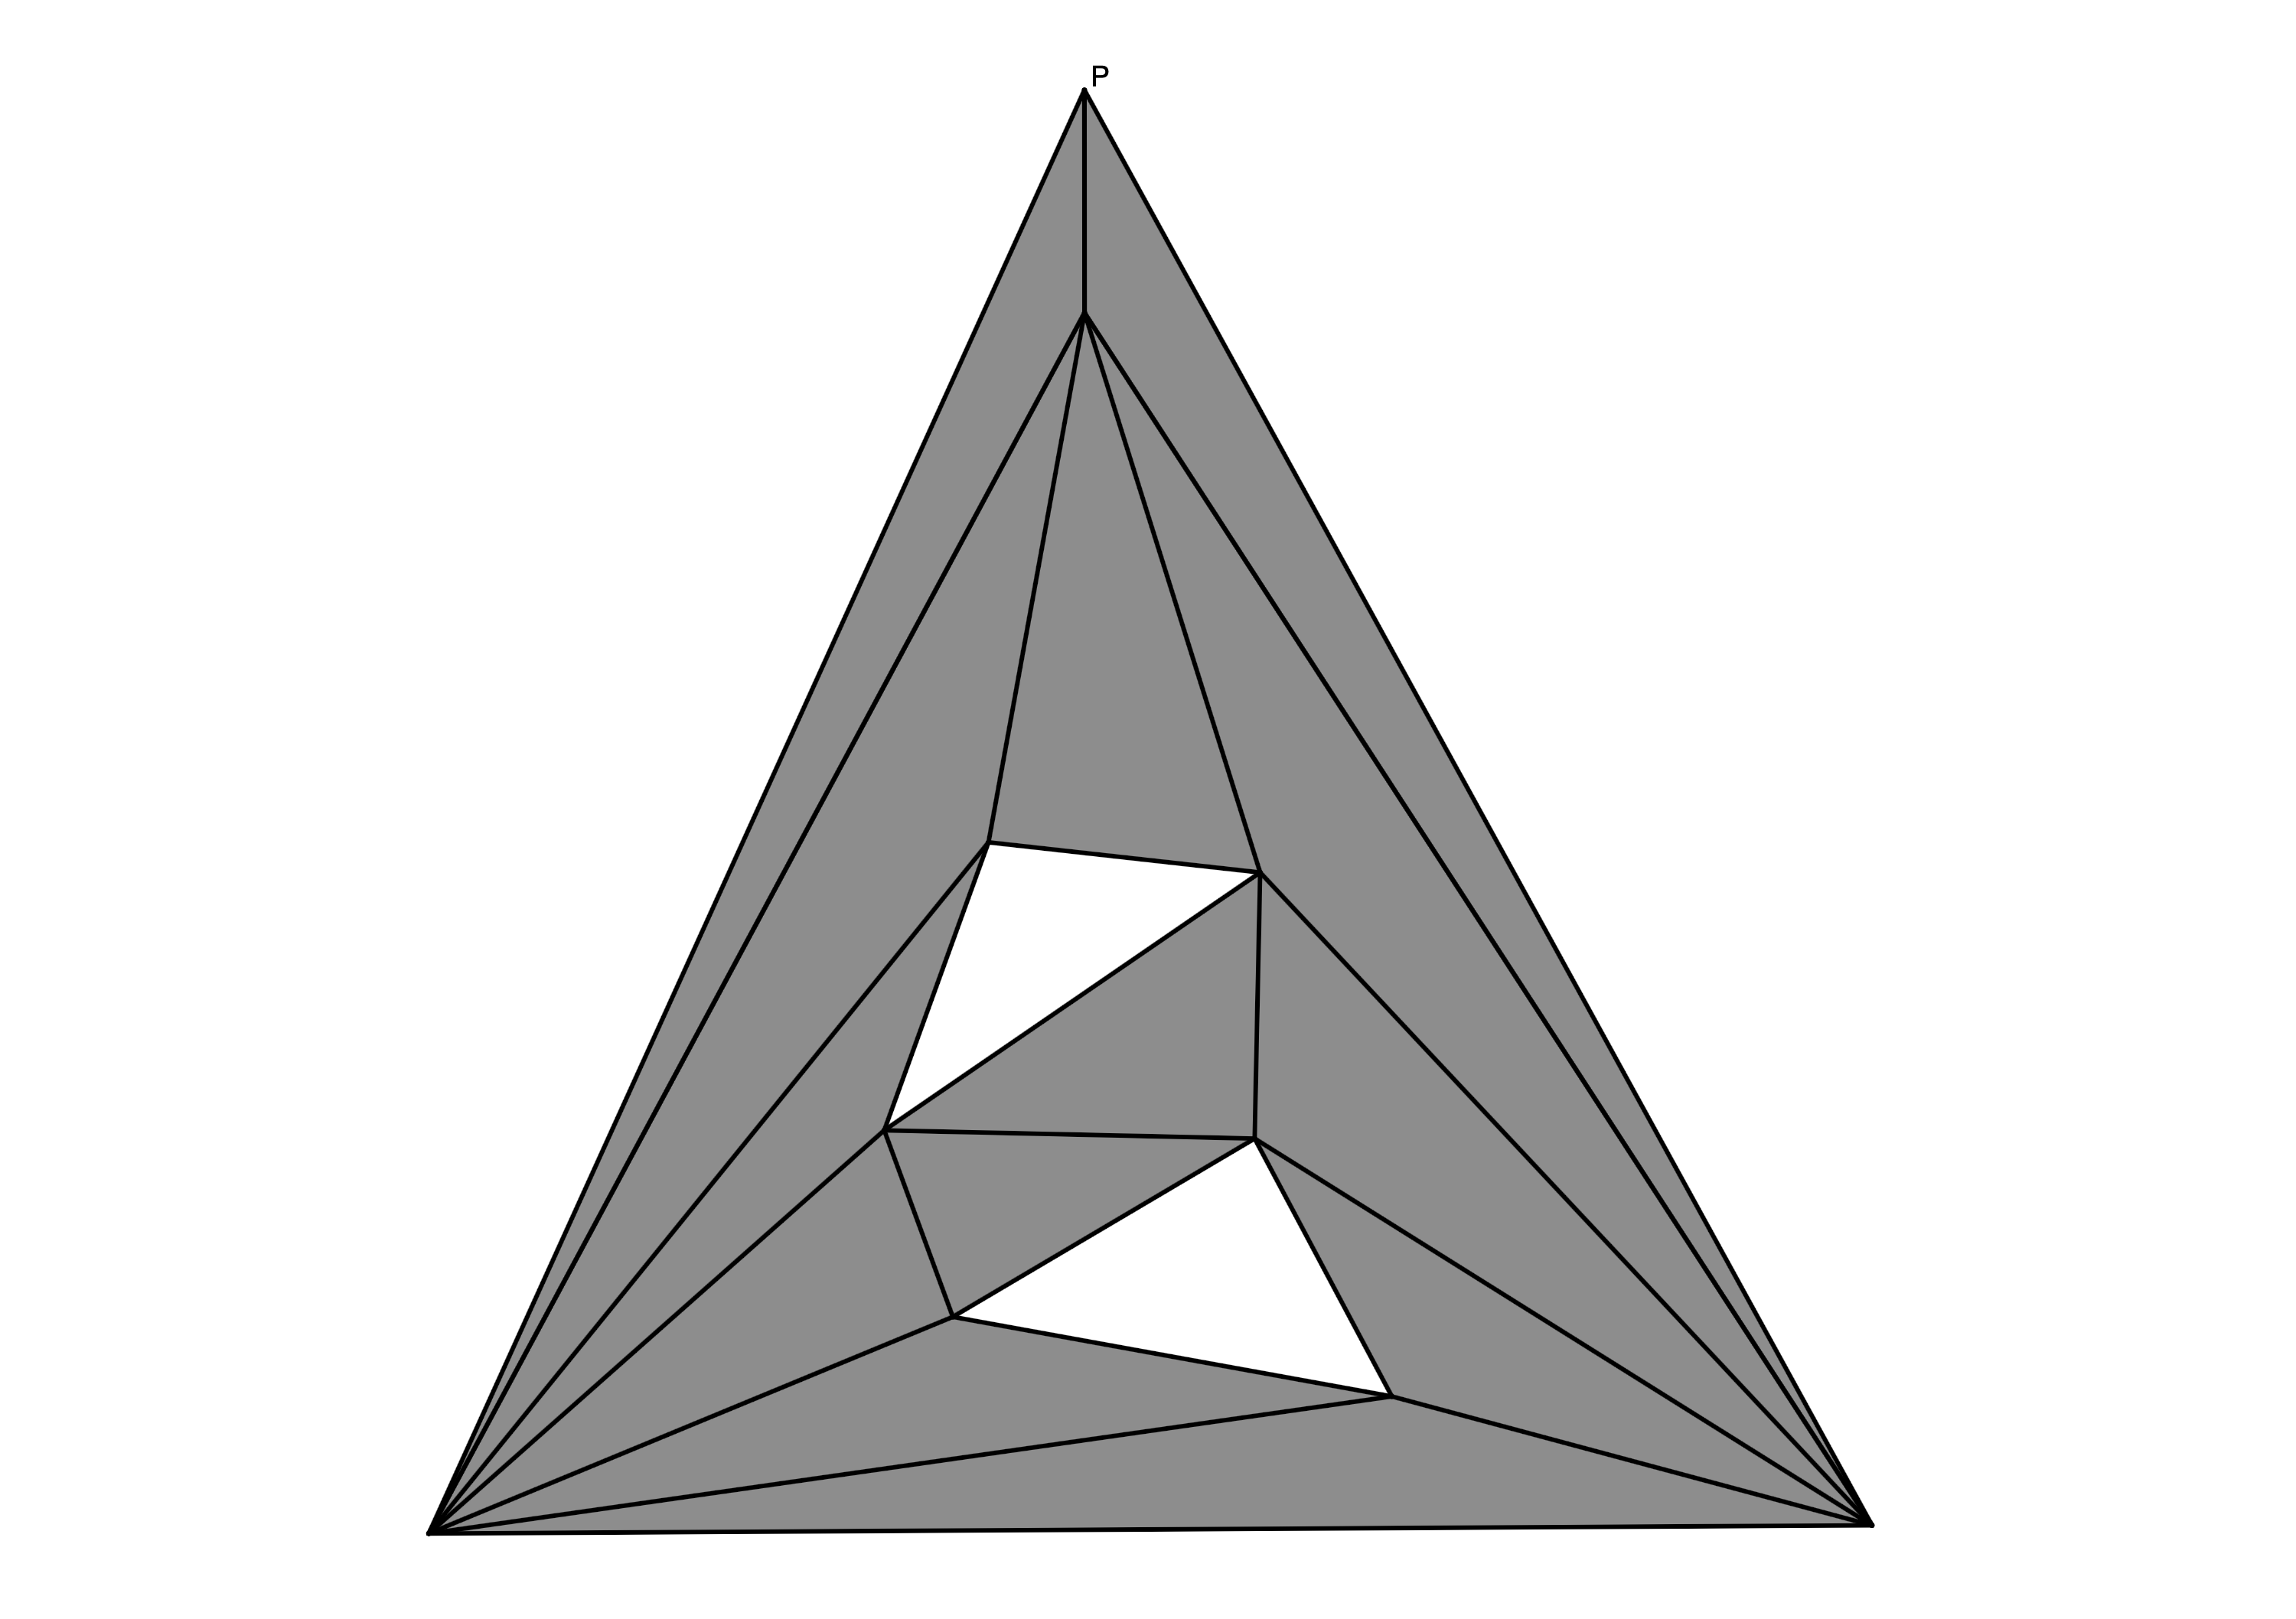
\includegraphics[width=.4\textwidth]{geogebra-export-9.png}}
        \caption{Polygons $P_{10}$ with $n=10$ vertices and $h=2$ holes} 
        \label{fig:p10}
      \end{figure}

    \item We make the observation that a triangulated polygon with holes forms a connected planar graph. Hence it will adhere to Euler's formula for planar graphs with equality:
    \begin{equation*}
      V - E + F = 2
    \end{equation*}
    where $V$, $E$ and $F$ are the number of vertices, edges and faces in the planar graph respectively. 
    Note that the outer face of a planar graph is also counted. 

    We will denote the number of triangles in the triangulation of a polygon as $t$. \\

    \begin{theorem}
      Any triangulation of a polygon $P$ with $n$ vertices and $h$ holes consists of $t = n+2h-2$ triangles.
    \end{theorem}
    \begin{proof}
      The number of vertices in the planar graph is equal to $n$ the number of vertices in the polygon. 
      \begin{equation*}
        V = n
      \end{equation*}
      The number of faces in the planar graph is equal to the sum of the number of triangles in the triangulation $t$, the number of holes $h$ and 1 for the exterior face.
      \begin{equation*}
        F = t + h + 1
      \end{equation*}
      Every triangle in the triangulation consists of three edges that are also edges of the planar graph. 
      If we add the edges that make up the outer and inner boundaries of the polygon $n$, we have counted every edge in the planar graph twice. Therefore:
      \begin{equation*}
        E = \frac{3t+n}{2}
      \end{equation*}
      By Euler's theorem for connected planar graphs we find that:
      \begin{align*}
        V - E + F &= 2 \\
        n - \frac{3t+n}{2} + t + h + 1 &= 2 \\
        n + 2h - 2 & = t \\
      \end{align*}

      Therefore the number of triangles in any triangulation of polygon $P$ with $n$ vertices and $h$ holes consists of $t=n+2h-2$ triangles.
    \end{proof}
  \end{enumerate}

  \begin{question}
    Let $p \in \R^2$ be a point, and let $S$ be a set of $n$ disjoint
    line segments in the plane. You may assume that the set containing
    $p$ and all endpoints of the segments in $S$ has no three colinear
    points (and thus $p$ does not lie on any of the segments).

    \begin{subquestions}
      \subquestion[20] Develop an algorithm to compute the length of a
      longest line segment $\overline{pq}$ that does not properly
      intersect the interior of any segment in $S$. (Recall that two
      segments properly intersect if and only if their interiors
      intersect). If segment $\overline{pq}$ does not exist your
      algorithm should return $\infty$. Prove that your algorithm is
      correct and analyze its running time.

      Note: the number of points rewarded for this question will
      depend on the running time of your algorithm.

      \subquestion[5] Is your algorithm still correct if the segments
      in $S$ may intersect? If so, argue why, if not, give an example
      why not, and describe how to fix it. You do \emph{not} have to
      argue about the running time of your algorithm in this scenario.
    \end{subquestions}

  \end{question}

  %  My answers for Q3 here...

  \begin{enumerate} 
    \item We start with the following observation:
    \vspace{0.3cm}
    \begin{theorem}
      If segment $\overline{pq}$ exists, then $q$ must lie on some segment $x \in S$
    \end{theorem}
    \begin{proof}
      Suppose for contradiction that $\overline{pq}$ exists, but $q$ does not lie on any segment $x \in S$.
      Then by assumption we know that $\overline{pq}$ is the longest line segment that does not properly intersect the interior of any of the $n$ segments in $S$.
      Then we can increase the length of $\overline{pq}$ by moving $q$ further from $p$ along the supporting line of $\overline{pq}$.
      However, since we don't want to create a proper intersection with one of the segments in $S$, we stop moving $q$ until it lies on one of the segments in $S$.
      If we could extend $\overline{pq}$ to a longer segment then $\overline{pq}$ was not the longest segment to fit the critera and therefore, $q$ must lie on some of the $n$ segments in $S$.
    \end{proof} 
    \vspace{0.3cm}
    \begin{theorem}
      If segment $\overline{pq}$ exists, then $\overline{pq}$ must pass through one of the endpoints of some segment $y \in S$
    \end{theorem}
    \begin{proof}
      Suppose for contradiction that $\overline{pq}$ exists, but it does not pass through one of the endpoints of any segment $y \in S$.
      By Theorem 2. we know that $q$ must lie on some line segment $x \in S$. And by assumption we know that $\overline{pq}$ does not properly intersect any of the segments in $S$.
      We will show that there is always at least one direction to move $q$ in on the segment $x$ so that the length of $\overline{pq}$ is increased.
      Suppose $\overline{pq}$ is orthogonal to $x$. Then moving $q$ in either direction on $x$ will strictly increase the length of $\overline{pq}$.
      If $\overline{pq}$ is not orthogonal to $x$, $\overline{pq}$ can be extended by moving $q$ on $x$ in the direction away from the orthogonal projection of $p$ on $x$.
      In both cases, moving $q$ in at least one direction which increases the length of $\overline{pq}$ is possible since $\overline{pq}$ does not properly intersect any segment in $S$ and does not pass through any endpoint of a segment in $S$.
      However, we can only move so far until $\overline{pq}$ will pass through an endpoint of a segment in $S$. Moving further would result in proper intersection.
      If we can extend $\overline{pq}$ to a longer segment then $\overline{pq}$ was not the longest segment to fit the critera and therefore, $\overline{pq}$ must pass through one of the endpoints of some segment in $S$.
    \end{proof}

    Since $\overline{pq}$ must pass through one the endpoints of a segment in $S$, we start by creating all the $2n$ halflines, from $p$ through both endpoints of every segment in $S$.

    \textbf{Algorithm Description} \\
    Sort all the segments based on their distance to $p$ in ascending order.
    During the course of the algorithm the plane $\mathbb{R}^2$ will be divided in regions defined as the area between 2 halflines going through $p$.
    We will use a balanced binary search tree to store these regions along with the segment in $S$ that bounds it.

    Then we iterate through each segment in ascending order and create the two halflines through $p$ and their two endpoints.

    There are 5 possible cases that can occur:
    \begin{enumerate}
      \item both endpoints are in the same unbounded regions. In this case we store the halflines along with the segment that bounds it in the search tree
      \item one endpoint falls in an existing bounded region $x$, while the other endpoint falls in some unbounded region.
       In this case we store the halfline together with the already existing halfline that defines $x$ on the side that the unbounded region is.
      We update the longest segment $\overline{pq}$ to be the edge between the intersection of the current segment that is being added and the halfline between the bounded and unbounded region.
      \item both endpoints fall in the same already bounded region. In this case we don't have to do anything
      \item both endpoints fall in different already bounded regions. In this case we have to check if there are any unbounded regions between these bounded regions.
      If there are, change them to regions bounded by the current segment being added. Then update the longest segment $\overline{pq}$ to be the edge between the intersection of the current segment being added and the halfline. 
      If there are multiple halflines, we only store the largest one.
      \item both endpoints fall in different unbounded regions. In this case we remove the old bounded region and add the new one like in case 1. 
      If there are any old segments bounding regions between the unbounded regions, these are not relevant anymore. We just need to know the region is bounded by some segment.
    \end{enumerate}
    After all segments have been added, we check if there are any unbounded regions left. If there are, we return $\infty$. 
    If all regions are bounded, we returned the longest segment $\overline{pq}$ that was stored.

    \textbf{Algorithm Running Time} \\
    This algorithm runs in $O(n \log n)$. Querying in the balanced binary can be done in $O(\log n)$ time. Handling any of the cases can be done in $O(\log n)$ time.
    Since we do this for every segment we add the total algorithm takes $O(n\log n)$ time.

    \item No this doesn't work if intersections are allowed. It could be fixed by adding not just the endpoints of the segments as points of interest but also adding the intersections points between the segments.
    This is because $q$ could be positioned on the intersection of two segments in $S$.
  \end{enumerate}
  

  \begin{question}[20] Let $P$ be a simple polygon with $n$ vertices,
    and let $\Delta$ be an equilateral triangle with corners $u$, $v$, and
    $w$, with $\overline{uv}$ horizontal and of length one, and with $w$
    above $\overline{uv}$.

    Sketch an $O(n^2\log n)$ time algorithm to test if there is a
    translation $\Delta^*$ of $\Delta$ that is completely contained in $P$,
    i.e. such that $\Delta^* \subseteq P$.

    Argue briefly that your solution is correct and achieves the
    stated running time. However, you do not have to give the full
    proof(s).

  \end{question}

  %  My answers for Q4 here...
  Let $\nabla$ denote the triangle $\Delta$ rotated 180 degrees.
  Note that the translation of the triangle $\Delta$ is completely defined by a single reference point $r$. This can be any point in the triangle but for convenience we use the top vertex.


  The approach we'll use is to find for every edge $e$ (connecting vertices $v_1$ and $v_2$ of $P$) of $P$ the region that $r$ can not be placed in due to one or more edges of $\Delta$ intersecting $e$.
  Every edge of $P$ will result in such regional constraints. If there remains a nonempty region in $P$ that adheres to all the edge constraints, the $r$ can be placed here so that $\Delta$ doesn't intersect any edges of $P$ and is fully contained in $P$.

  Imagine two copies of $\nabla$, $\nabla_1$ (vertices $x_1, x_2, x_3$) and $\nabla_2$ (vertices $y_1, y_2, y_3$), with their bottom points coinciding with $v_1$ and $v_2$ respectively. 
  Also imagine edges connecting $x_1$ to $y_1$, $x_2$ to $y_2$, and $x_3$ to $y_3$. 
  Note that the bottom edge here will correspond to $e$. 
  Let $A_e$ denote the polygon defined by the vertices $x_1, x_2, x_3, y_1, y_2, y_3$.
  Placing $r$ anywhere within $A$ will result in one or more edges of $\Delta$ being intersected by $e$. If $r$ is positioned outside of $A$, none of the edges of $\Delta$ intersect $e$.

  We can define such a polygon $A_e$ for every edge $e$ in $P$. 
  $A$ will then give the region in which we cannot place $r$ and is defined as:
  $$A = \bigcup_{e \in \text{edges}(P)} A_e$$
  
  Following this, a simple set difference, $F = P - A$ will give the feasible region inside $P$ where we can place $r$ so that $\Delta$ is fully contained in $P$.
  If $F = \varnothing$, we return that there is no $\Delta^*$, else we return there is a $\Delta^*$.

  % Performing boolean operations on pylgons with $n$ vertices takes $O(n\log n + k\log n)$ where $k$ is the number of intersection points.
  Creating a single $A_e$ using map overlay can be done in $O(n\log n)$ since the number of intersection points is linear in the number of vertices, $k = O(n)$.
  This is because $A_e$ has a constant number of vertices and therefore edges.
  Since we have $n$ edges and therefore $n$ $A_e$'s, creating the map overlay will take $O(n^2\log n)$. The final set difference can be done in constant time since the map overlay has already been created.

\end{document}
